\subsection{Aplicação Fábrica: Registo de Saída de Produto Acabado}
\subsubsection*{Descrição do caso de uso}
No registo de produto acabado, espera-se que utilizador entre na página e indique o código de barras do produto acabado. A informação da data deve ser indicada automaticamente pelo sistema. A partir da segunda fase do projeto deverá ainda existir um campo para indicar o cliente.

\begin{figure}[H]
	\centering
	
	\begin{subfigure}[t]{0.45\linewidth}
		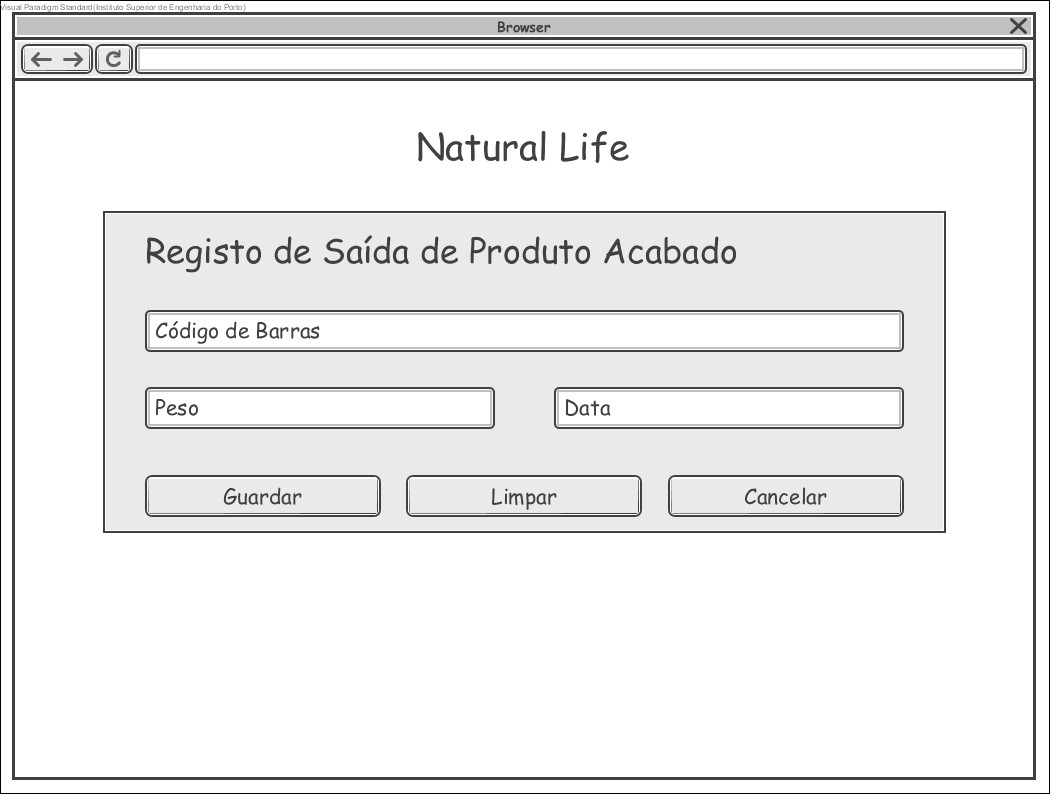
\includegraphics[width=\linewidth]{figuras/Diagramas_vp/DI_Fabrica_5_Saida_de_Produto_Acabado_1_Fase.jpg}
		\label{fig:di_saida_prod_acabado_1}
		\caption{Após concluir primeira fase}
	\end{subfigure}
	\begin{subfigure}[t]{0.45\linewidth}
		\includegraphics[width=\linewidth]{figuras/Diagramas_vp/DI_Fabrica_5_Saida_de_Produto_Acabado_2_Fase.jpg}
		\label{fig:di_saida_prod_acabado_2}
		\caption{Após concluir segunda fase}
	\end{subfigure}
	
	\caption{Modelo do menu}
	\label{fig:di_saida_prod_acabado}
\end{figure}

\subsubsection*{Fluxo do caso de uso (2ª fase)}
O caso de uso inicia-se com a abertura da página do registo de saída de produto acabado. É apresentado o formulário com a data previamente preenchida. O utilizador tem de indicar o código de barras do produto acabado e o ID do cliente de uma lista dropdown.  Após indicar as informações solicitadas precisona o botão "Guardar". No final do registo é apresentada uma mensagem ao utilizador. Caso o registo seja feito com sucesso um novo separador é aberto com o código de barras para ser impresso.


\begin{figure}[H] 
	\begin{center}
		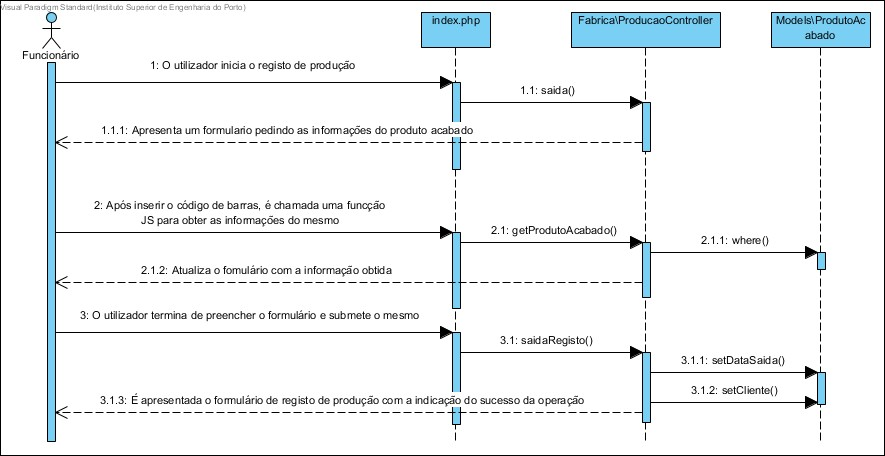
\includegraphics[width=0.95\textwidth,keepaspectratio]{figuras/Diagramas_vp/SD_Fabrica_5_Saida_de_Produto_Acabado.jpg}
		\caption{Diagrama de sequência registo de produto acabado}
		\label{fig:sd_saida_prod_acabado} 
	\end{center}
\end{figure}